\section{Results and Discussion}

\subsubsection*{1. Experimental Setup}

Two metallic electrodes—brass and steel—were analyzed using DropSens instrumentation. The Open Circuit Potential (OCP) was measured with a multimeter:
\begin{itemize}
  \item Brass: OCP = \( -142.9\,\text{mV} \)
  \item Steel: OCP = \( -441\,\text{mV} \)
\end{itemize}

A potential sweep of ±200 mV around the OCP was applied at a scan rate of 1 mV/s. The electrode area was 0.28274 cm\(^2\) in both cases.

\vspace{0.2cm}
\subsubsection*{2. Brass Electrode Results}

The Tafel curve for brass was processed from the experimental data. Linear regression was applied to the anodic and cathodic regions to extract corrosion parameters.

\begin{itemize}
    \item \textbf{Corrosion potential:} \( E_{\text{corr}} = -0.258 \) V
    \item \textbf{Corrosion current density:} \( j_{\text{corr}} = 5.40 \times 10^{-6} \) A/cm\(^2\)
    \item \textbf{Anodic fit:} \( \log(j) = 11.842 \cdot E + 1.646 \)
    \item \textbf{Cathodic fit:} \( \log(j) = -6.127 \cdot E - 6.460 \)
\end{itemize}

\begin{figure}[ht!]
    \centering
    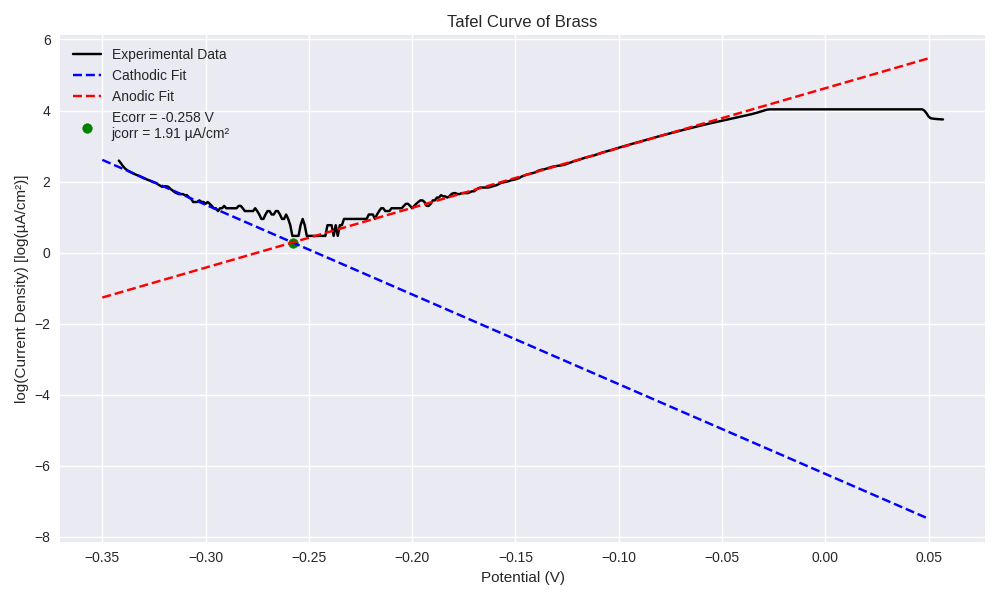
\includegraphics[width=0.7\linewidth]{Figures/TAFEL-BRASS.png}
    \caption{Tafel curve for brass electrode.}
    \label{fig:tafel_brass}
\end{figure}

\vspace{0.2cm}
\subsubsection*{3. Steel Electrode Results}

The steel electrode exhibited higher electrochemical activity. The corrosion parameters were extracted similarly:

\begin{itemize}
    \item \textbf{Corrosion potential:} \( E_{\text{corr}} = -0.388 \) V
    \item \textbf{Corrosion current density:} \( j_{\text{corr}} = 8.87 \times 10^{-5} \) A/cm\(^2\)
    \item \textbf{Anodic fit:} \( \log(j) = 13.650 \cdot E + 1.357 \)
    \item \textbf{Cathodic fit:} \( \log(j) = -5.696 \cdot E - 6.288 \)
\end{itemize}

\begin{figure}[ht!]
    \centering
    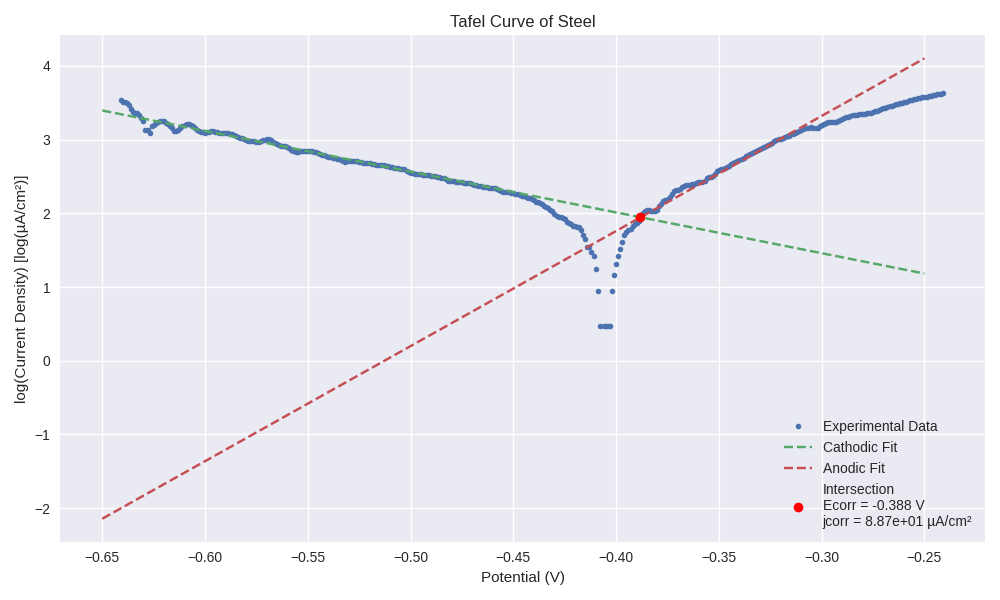
\includegraphics[width=0.7\linewidth]{Figures/TAFEL-STEEL.png}
    \caption{Tafel curve for steel electrode.}
    \label{fig:tafel_steel}
\end{figure}

\vspace{0.2cm}
\subsubsection*{4. Corrosion Penetration Rate (CPR) Calculation}

The CPR was calculated using the empirical formula:

\begin{equation}
\text{CPR} = \frac{0.13 \cdot j_{\text{corr}} \cdot \text{EW}}{\rho}
\end{equation}

Where:
\begin{itemize}
    \item CPR: Corrosion rate (mm/year)
    \item \( j_{\text{corr}} \): Corrosion current density (A/cm\(^2\))
    \item EW: Equivalent weight (g)
    \item \( \rho \): Density (g/cm\(^3\))
\end{itemize}

\vspace{0.2cm}
\textbf{Brass Parameters:}

Table~\ref{tab:cpr_brass} summarizes the main electrochemical parameters obtained for 
the brass electrode. These values were used to calculate the corrosion penetration rate (CPR).

\begin{table}[h!]
\centering
\caption{CPR calculation for brass}
\label{tab:cpr_brass}
\begin{tabular}{|c|c|}
\hline
Parameter & Value \\
\hline
\( j_{\text{corr}} \) & \( 5.40 \times 10^{-6} \) A/cm\(^2\) \\
EW & 50.42 g \\
\( \rho \) & 8.52 g/cm\(^3\) \\
CPR & \( 4.17 \times 10^{-5} \) mm/year \\
\hline
\end{tabular}
\end{table}

\vspace{0.2cm}
\textbf{Steel Parameters:}

Similarly, Table~\ref{tab:cpr_steel} presents the parameters obtained for the steel electrode, 
which show a higher corrosion current density and consequently a higher CPR compared to brass.

\begin{table}[h!]
\centering
\caption{CPR calculation for steel}
\label{tab:cpr_steel}
\begin{tabular}{|c|c|}
\hline
Parameter & Value \\
\hline
\( j_{\text{corr}} \) & \( 8.87 \times 10^{-5} \) A/cm\(^2\) \\
EW & 55.845 g \\
\( \rho \) & 7.85 g/cm\(^3\) \\
CPR & \( 8.23 \times 10^{-4} \) mm/year \\
\hline
\end{tabular}
\end{table}


\vspace{0.2cm}
\subsubsection*{5. Discussion of Results}

The steel electrode exhibited a significantly higher corrosion current density and CPR compared to brass, indicating lower corrosion resistance under the same conditions. The brass electrode showed a flatter Tafel slope and lower \( j_{\text{corr}} \), suggesting more stable electrochemical behavior. These results align with the expected performance of brass in mildly aggressive environments.

The corrosion experiments were conducted in a controlled electrochemical cell using a 0.5 M hydrochloric acid (HCl) solution as the corrosive medium. The presence of chloride ions (\( \text{Cl}^- \)) accelerates the breakdown of passive layers on metal surfaces, promoting localized corrosion and pitting.

The potentiodynamic scans revealed distinct corrosion behaviors:
\begin{itemize}
    \item \textbf{Steel} exhibited a higher corrosion current density and a more negative corrosion potential, indicating greater susceptibility to acid attack.
    \item \textbf{Brass} showed lower current densities and a more stable potential, suggesting better resistance in chloride-rich environments.
\end{itemize}

These differences can be attributed to the alloy composition and surface reactivity. Brass, being a copper-zinc alloy, benefits from the formation of protective oxides and its lower standard electrode potential. Steel, composed primarily of iron, readily oxidizes in acidic media, forming soluble iron ions and unstable corrosion products.

\vspace{0.2cm}
\textbf{Limitations and Considerations:}
\begin{itemize}
    \item The corrosion rates calculated are specific to the 0.5 M HCl medium and may differ significantly in neutral or alkaline environments.
    \item The extrapolation of Tafel lines assumes ideal linearity, which may not fully capture complex surface phenomena such as passivation or film formation.
    \item The reference electrode potential must be corrected if comparing results to literature values based on other reference systems (e.g., NHE).
\end{itemize}
